\documentclass{sigplanconf}

% The following \documentclass options may be useful:

% preprint      Remove this option only once the paper is in final form.
% 10pt          To set in 10-point type instead of 9-point.
% 11pt          To set in 11-point type instead of 9-point.
% authoryear    To obtain author/year citation style instead of numeric.

\usepackage{tikz}
\usepackage{amsmath}
\usepackage{graphicx}
\usepackage{xspace}
\usepackage{hyperref}
\hypersetup{
    bookmarks=false,        % show bookmarks bar?
    unicode=false,          % non-Latin characters in Acrobat’s bookmarks
    pdftoolbar=true,        % show Acrobat’s toolbar?
    pdfmenubar=true,        % show Acrobat’s menu?
    pdffitwindow=false,     % window fit to page when opened
    pdfstartview={FitH},    % fits the width of the page to the window
    pdftitle={My title},    % title
    pdfauthor={Author},     % author
    pdfsubject={Subject},   % subject of the document
    pdfcreator={Creator},   % creator of the document
    pdfproducer={Producer}, % producer of the document
    pdfkeywords={keyword1} {key2} {key3}, % list of keywords
    pdfnewwindow=true,      % links in new window
    colorlinks=true,        % false: boxed links; true: colored links
    linkcolor=black,        % color of internal links (change box color with linkbordercolor)
    citecolor=black,        % color of links to bibliography
    filecolor=black,        % color of file links
    urlcolor=black          % color of external links
}

\def \JCP{JCP\xspace}
\def \SUN{\mbox{Sun Microsystems}\xspace}
\def \ORACLE{\mbox{Oracle}\xspace}
\def \DALVIK{\mbox{Dalvik}\xspace}
\def \Jsr{JSR\xspace}
\def \JSR{\Jsr 292\xspace}
\def \GOOGLE{\mbox{Google}\xspace}
\def \ANDROID{\mbox{Android}\xspace}
\def \JVM{JVM\xspace}
\def \DEX{\mbox{DEX}\xspace}
\def \VM{VM\xspace}
\def \BSM{BSM\xspace}

\newcommand{\executeiffilenewer}[3]{%
  \ifnum\pdfstrcmp{\pdffilemoddate{#1}}{\pdffilemoddate{#2}}>0%
  {\immediate\write18{#3}}\fi%
}

\newcommand{\includesvg}[1]{%
  \executeiffilenewer{#1.svg}{#1.pdf}{inkscape -z -D --file=#1.svg --export-pdf=#1.pdf --export-latex}%
  \input{#1.pdf_tex}%
}

\newcommand{\tinyline}[3]{
  \tiny #1 &
  \tiny #2 &
  \tiny #3\\
  \hline
}

\newenvironment{listminimal}[1]%
{ \begin{minipage}{#1}%
    \medskip
    \begin{list}%
      {}%
      {%
        \setlength{\labelwidth}{0pt}%
        \setlength{\leftmargin}{0pt}%
        \setlength{\itemsep}{1pt}%
        \setlength{\parskip}{0pt}%
        \setlength{\parsep}{0pt}}%
}%
{ \\ \end{list} \end{minipage} }

\newcommand{\fixme}[1]{{\color{red} // FIXME #1}\\}

\begin{document}

\special{papersize=8.5in,11in}
\setlength{\pdfpageheight}{\paperheight}
\setlength{\pdfpagewidth}{\paperwidth}

\conferenceinfo{PPPJ '14}{Month d--d, 20yy, City, ST, Country} 
\copyrightyear{2014} 
\copyrightdata{978-1-nnnn-nnnn-n/14/mm} 
\doi{nnnnnnn.nnnnnnn}

% Uncomment one of the following two, if you are not going for the 
% traditional copyright transfer agreement.

%\exclusivelicense                % ACM gets exclusive license to publish, 
                                  % you retain copyright

%\permissiontopublish             % ACM gets nonexclusive license to publish
                                  % (paid open-access papers, 
                                  % short abstracts)

\titlebanner{banner above paper title}        % These are ignored unless
\preprintfooter{short description of paper}   % 'preprint' option specified.

\title{Title Text}
\subtitle{Subtitle Text, if any}

\authorinfo{Roussel Gilles}
           {University Paris-Est Marne-la-Vallee}
           {roussel@univ-mlv.fr}
\authorinfo{Forax Remi}
           {University Paris-Est Marne-la-Vallee}
           {forax@univ-mlv.fr}
\authorinfo{Pilliet Jerome}
           {University Paris-Est Marne-la-Vallee}
           {pilliet@univ-mlv.fr}

\maketitle

\begin{abstract}
This is the text of the abstract.

bla bla bla bla bla bla bla bla bla
bla bla bla bla bla bla bla bla bla
bla bla bla bla bla bla bla bla bla
bla bla bla bla bla bla bla bla bla
bla bla bla bla bla bla bla bla bla
bla bla bla bla bla bla bla bla bla
bla bla bla bla bla bla bla bla bla

bla bla bla bla bla bla bla bla bla
bla bla bla bla bla bla bla bla bla
bla bla bla bla bla bla bla bla bla
bla bla bla bla bla bla bla bla bla
bla bla bla bla bla bla bla bla bla
bla bla bla bla bla bla bla bla bla
bla bla bla bla bla bla bla bla bla
\dots
\end{abstract}

\category{CR-number}{subcategory}{third-level}

% general terms are not compulsory anymore, 
% you may leave them out
\terms
term1, term2

\keywords
keyword1, keyword2

  \section{Android}

    \ANDROID is the mobile operating system of Google.
    It's an open-source project called ``\ANDROID Open-Source Project'' (AOSP).
    In Q2 2013, \ANDROID occupies almost 80\% of the market share with more than 187 million units shipped \cite{idc-website}.
    The success of \ANDROID can be explain by an open project and an open market
    which are very attractive for devices producers, service providers and application developers \cite{ieee-butler-android-landscape}.

    \ANDROID mainly run on embedded environments like smartphones and tablets.
    Therefore, strong constraints apply to \ANDROID
    and it have to support ARM architecture and now Intel architecture.
    
    Even if hardware of devices which supports \ANDROID becomes more efficient,
    devices can't be as efficient as a desktop computer because of miniaturization of devices.
    Being a mobile device requires a minimal energetic consumption.
    Moreover, \ANDROID is portable and it must be adaptable to different devices.
    Forcing it to abstract itself from hardware.

    The \ANDROID architecture is described like a ``software stack'' (fig. \ref{ASA}).
    It's composed to:
    \begin{itemize}
      \item a modified version of the Linux kernel.
        It offers an hardware abstraction,
        an existing memory and process managements
        and a security and networking models;
      \item native libraries (C/C++)
        which provide most of features of the \ANDROID system;
      \item a virtual machine called ``\DALVIK''. \DALVIK is a important component of \ANDROID.
        It runs applications converted into the \DEX format.
        \DALVIK uses a core API written from scratch in Java
        which can be assimilate to the version 5 or 6 of the Java API;
      \item an application framework to enable the making of \ANDROID applications;
      \item and some default applications.
    \end{itemize}

    \subsection{Differences between the JVM and Dalvik}

      The main difference between these two machines is that \DALVIK is a register based machine while the \JVM is stack based.
      A stack based VM uses more instructions to manipulate data and to implement Java code than a register based VM.
      But the register based VM instructions tends to be larger \cite{ieee-paul-kundu-energy-perspective}

      The bytecode Java is given in a ``.class'' file and only contains the code of one class (fig. \ref{SJA}).
      The file is made of a series of tables, which contains various information, the code of the class and some other things.
      The code contains references to these tables.
      Among these tables, one is the table of constants (constant-pool).
      This table stores most of the constant values of the class (numbers or texts)
      and more evolved elements (data types, class names, attribute names, \dots).

      \begin{figure}[h]
        \centering \includegraphics[width=\columnwidth]{structure-jar-apk.png}
        \caption{structure of JAR and APK files}
        \label{SJA}
      \end{figure}

      Whereas, \DEX format contains all the code of the application (fig. \ref{SJA}).
      It will be loaded in one piece.
      It is a read-only format, so the code can't be changed at runtime.
      Duplicate constants such as strings used in multiple class files
      are included only once in the \DEX file to save space.
      Unlike the \JVM, \DALVIK uses one constant-pool by type of constant
      except for the primitive types which are directly encoded with the opcode.
      It means more smaller indexes for instructions.\\

      \begin{figure}[t]
        \centering \includegraphics[width=\columnwidth]{dex-tools-chain.png}
        \caption{\ANDROID application tools-chain}
        \label{DTC}
      \end{figure}

      \DALVIK cannot directly execute Java bytecode.
      It have first to translate the Java byte code to a \DALVIK specific bytecode called \DEX
      and It cans optimize its bytecode (\mbox{ODEX}) to save space (fig. \ref{DTC}).


    \begin{figure}[!h]
      \centering \def\svgwidth{\columnwidth} \includesvg{android-system-architecture}
      \caption{android system architecture \cite{wiki-android}}
      \label{ASA}
    \end{figure}

  \section{Java Specification Request 292}

    The \JSR is a request from \JCP and led by \SUN in 2006.
    It had been integrated in 2011 in the version 7 of Java,
    modifying both the Java language specification and the \JVM specification.

    Since late 90's, a lot of language
    implementors have chosen the JVM as their target platform \cite{wiki-jvm-lang},
    for several reasons among the size of the ecosystem,
    the presence of mature GCs and Just In Time compilers. 

    The aim of this \Jsr is to ease the implementation of dynamically typed languages
    by providing a new way to do function calls that allows language implementors
    to specify a specific semantics, independantly of the semantics of the language Java.
    
    This \Jsr is composed of two parts, the first part, specifies the semantics of
    new opcodes. The second part defined an API, java.lang.invoke that allows
    to create runtime typesafe function pointers (java.lang.invoke.MethodHandle) and
    methods to combine those function pointers to do thing like function composition,
    function argument permutation, etc.

    The next sections will present the new API and new instructions but before
    we want to introduce an example that we will use for the rest of the paper.

    \subsection{Example}
      Let suppose we have the following code in Groovy \cite{lang-groovy}

      {\scriptsize \begin{verbatim}
  def foo(a) {
    a + 2
  }

  println foo(9)
  println foo("test")
\end{verbatim} }


      It prints 11 and test2. For the fist call to foo, 'a' is an integer so the function + refers
      to the function +(int,int) while for the second call to foo, 'a' is a string, so the
      function + refers to the function +(String,String).

      If one try to translate that code in Java bytecode, it will be something like

      {\tiny \begin{verbatim}
  def foo(a) {
    aload 0   // 0 is offset of first variable, 'a' here
    iconst_2  // load the integer constant 2
    invokevirtual Object + (I)LObject;
    areturn 
  }
\end{verbatim} }


      As you can see, the Java bytecode is typed, each instruction is prefixed 
      by the type of the operand ('a' for object, 'i' for integer, etc)
      and the method call (invokevirtual) specify the type of the receiver and its parameter ;
      an object (java/lang/Object) followed by an integer (I) ; and its return type
      which is also an object in the example.

      The code above doesn't work because invokevirtual is an existing Java bytecode that call
      a virtual method using the Java semantics so the Virtual Machine or more precisely
      the bytecode verifier will check that there is a method '+' on java.lang.Object
      that takes an integer and returns an Object. If you have used Java, you already know
      that this method doesn't exist. So the bytecode verification will fail.

      Another possible translation is to use a cascade of if ... instanceof.

      {\tiny \begin{verbatim}
  static Object plus(String v, Object v2) {
    return v.concat(String.valueOf(v2));
  }

  static Object plus(int v, int v2) {
    return Integer.sum(v, v2)
  }

  static Object foo(Object v, int i) {
    if (v instanceof Integer) {
      return plus((Integer)v, i);
    }
    if (v instanceof String) {
      return plus((String)v, i);
    }
    throw new Error();
  }

  public static void main(String[] args) {
    System.out.println(foo(9));
    System.out.println(foo("bar"));
  }
\end{verbatim} }


      While this code works, it supposes that all possible variations of + are known at compile time,
      something which is not true in most dynamic languages (Ruby, Groovy, Dart by example).
      This code can also be slow because for real languages, the number of if ... instanceof branches
      can be greater than a dozen. 
      
      To solve these issues, the \Jsr introduces a new bytecode named invokedynamic with no predefined
      linking semantics and a mechanism that allows to specify the linking semantics in Java
      or any languages that can be compiled to bytecodes.
      Invokedynamic is a function call so it can simulate every other existing Java calls that delegate
      its linking semantics to an external Java method, the bootstrap method.
      The bootstrap method is called the first time the invokedynamic opcode is encounter by the interpreter,
      with the context where the opcode is located i.e.
      the declaring class (encapsulated in a java/lang/invoke/Lookup object), a symbolic name,
      the declared parameter types as a java/lang/invoke/MethodType and return
      a CallSite object which is a box that contains a function pointer (a java/lang/MethodHandle).
      Any subsequent execution of the invokedynamic opcode will call the function pointer
      stored inside the callsite object returned by the bootstrap method.
      
      For our example, the code of foo with invokedynamic is

      \newpage
      {\tiny \begin{verbatim}
  def foo(a) {
    aload 0
    iconst_2 
    invokedynamic  + (LObject;I)LObject;
      bsm: invokestatic RT.bootstrap:(LMethodHandles$Lookup;LString;LMethodType;)LCallSite;
    areturn 
  }
\end{verbatim} }

      The first time that foo is executed, the method bootstrap of the class RT will be called, with a lookup corresponding to the class containing foo,
      with ``+'' as string and a MethodType corresponding to the descriptor ``(Ljava/lang/Object;I)Ljava/lang/Object;''.% (cf. \ref{FOOBSM}).

      {\scriptsize \begin{verbatim}
import static java.lang.invoke.MethodType.*

public class RT {
    ...
  private static final Lookup lookup = MethodHandles.lookup();

  public static CallSite bootstrap(
      Lookup caller, String name, MethodType type)
      throws IllegalAccessException, NoSuchMethodException {
    MethodType mt = methodType(Object.class,
                               MutableCallSite.class,
                               Object[].class);
    MethodHandle mh =
      lookup.findStatic(BootStraps.class, "change", mt);
    return new CSMutableBind(type, mh);
  }
    ...
}
\end{verbatim} }


      Moreover, invokedynamic comes with an API that allow to create several data pattern
      dynamically and lazily like by example a tree of if ... instanceof branches.

    \subsection{Package java.lang.invoke}
      The \JSR has created a new package named ``java.lang.invoke''.
      It contains several classes to ease the implementation of dynamic languages support.
      These classes are directly understood by the \JVM.
      It is composed of classes MethodType, MethodHandle, CallSite and SwitchPoint.
      All classes answer to one or more problems coming from dynamic languages optimizations or implementations.

      \subsubsection{MethodType}
        A method type represents the arguments and return type accepted and returned by a method handle,
        or the arguments and return type passed and expected by a method handle caller.
        This class represents a method signature.

        {\tiny \begin{verbatim}
import static java.lang.invoke.MethodType.*

public class RT {
    ...
  private static final MethodHandle TARGET_INT;
  private static final MethodHandle TARGET_STRING;
  private static final MethodHandle TARGET_CHECK;

  static {
    try {
      TARGET_INT = lookup.findStatic(BootStraps.class, "plus", methodType(Object.class, int.class, int.class));
      TARGET_STRING = lookup.findStatic(BootStraps.class, "plus", methodType(Object.class, String.class, int.class));
      TARGET_CHECK = lookup.findStatic(BootStraps.class, "check", methodType(boolean.class, Object.class, Class.class));
    } catch (NoSuchMethodException|IllegalAccessException e) {
      throw new AssertionError(e);
    }
  }
    ...
}
\end{verbatim} }

        A method type is immutable, so this type can be created only by factory methods.
        In our example, we need three method types, one for each method we have to call:
        the ``check'' method; and the two methods ``plus''.

        {\scriptsize \begin{verbatim}
  private static Object plus(int a, int b) {
    return a + b;
  }

  private static Object plus(String a, int b) {
    return a + b;
  }

  private static boolean check(Object value, Class<?> clazz) {
    return value.getClass() == clazz;
  }

  private static final MethodHandle TARGET_INT;
  private static final MethodHandle TARGET_STRING;
  private static final MethodHandle TARGET_CHECK;

  static {
    try {
      MethodType mti = MethodType
          .methodType(Object.class, int.class, int.class);
      TARGET_INT =
        lookup.findStatic(BootStraps.class, "plus", mti);

      MethodType mts = MethodType
          .methodType(Object.class, String.class, int.class);
      TARGET_STRING =
        lookup.findStatic(BootStraps.class, "plus", mts);

      MethodType mtc = MethodType
          .methodType(boolean.class, Object.class, Class.class);
      TARGET_CHECK =
        lookup.findStatic(BootStraps.class, "check", mtc);
    } catch (NoSuchMethodException|IllegalAccessException e) {
      throw new AssertionError(e);
    }
  }
\end{verbatim} }


      \subsubsection{MethodHandle / MethodHandles}
        \label{MH}
        A method handle is a typed, directly executable reference to
        an underlying method, constructor, field, or similar low-level operation,
        with optional transformations of arguments or return values.
        This class represents a function pointer.
        A method handle can be create by different factory methods depending to the kind of method handle and accessibility.

        We can distinguish two kinds of method handle:
        the one which do a direct call to a method or to a field access, this method handle is final;
        and the one which manipulate arguments, they are called ``combinors''.
        The combinors contains at least one final method handle and can be represent by a tree.

        In our example, we want to call a method which takes an Object and an integer and which returns an Object: (Object,I)Object.
        We need to resolve which right method we have to call (addition or concatenation).
        To do that, we write a method which will create the right method handle called ``change'' (detailed after).

        We need to adapt arguments to move from an Object and an integer to a CallSite and an array of Object.
        So we convert arguments (asType), we collect them to form the array of Objects (asCollector) and we add the call site at first argument (bindTo).

        {\tiny \begin{verbatim}
public class RT {
    ...
  private static class CSMutableBind extends MutableCallSite {
    CSMutableBind(MethodType type, MethodHandle mh) {
      super(type);
      setTarget(mh.bindTo(this).asCollector(Object[].class, type.parameterCount()).asType(type));
    }
  }
    ...
}
\end{verbatim} }

        This adaptation form the method handles tree of the figure \ref{ast1}.

        % graph 1
        \begin{figure}[!h]
          \centering \resizebox{.6\linewidth}{!}{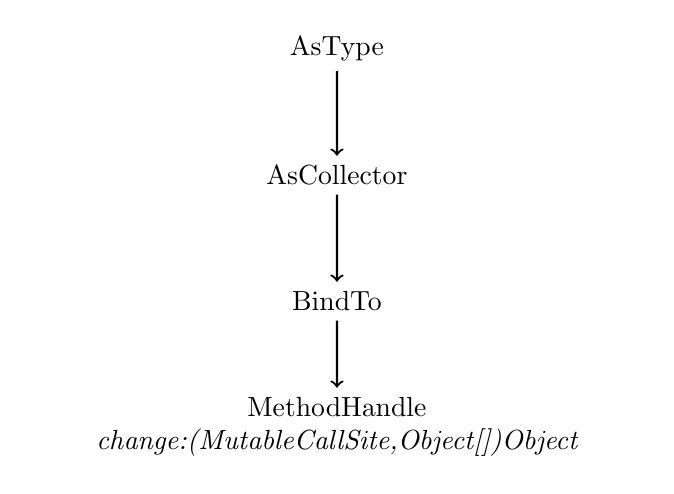
\begin{tikzpicture}[scale=1.6]
  \node[text width=3in,align=center](A1) at (2,-2){AsType};
  \node[text width=3in,align=center](A2) at (2,-3){AsCollector};
  \node[text width=3in,align=center](A3) at (2,-4){BindTo};
  \node[text width=3in,align=center](A4) at (2,-5){MethodHandle\\{\it change:(MutableCallSite,Object[])Object}};

  \draw[thick,->](A1) -- (A2);
  \draw[thick,->](A2) -- (A3);
  \draw[thick,->](A3) -- (A4);
\end{tikzpicture}
}
          \caption{method handles tree: bootstrap method call}
          \label{ast1}
        \end{figure}

        When the call site is created, the method handle tree is called, so the ``change'' method is called.

        {\scriptsize \begin{verbatim}
import static java.lang.invoke.MethodHandles.*;

public class RT {
    ...
  private static Object change(
      MutableCallSite callSite, Object[] arguments)
      throws Throwable {
    MethodHandle target;
    MethodType type = callSite.type();
    Class<?> aClass = arguments[0].getClass();
    if (aClass == Integer.class) {
      target = TARGET_INT.asType(type);
    } else if (aClass == String.class) {
      target = TARGET_STRING.asType(type);
    } else {
      throw new LinkageError("bad receiver class");
    }
    MethodHandle test =
      insertArguments(TARGET_CHECK, 1, aClass);
    test = dropArguments(test, 1, type.parameterType(1));
    callSite.setTarget(
      guardWithTest(test, target, callSite.getTarget()));
    return target.invokeWithArguments(arguments);
  }
    ...
}
\end{verbatim} }


        The method “change” takes a look to the dynamic type of ’a’ (let say it’s an integer),
        finds the corresponding implementation of the ``plus'' method,
        re-links a method handle tree representing by a combinor called ``GuardWithTest''.
        This combinor check the class of 'a',
        if the type of ’a’ is an integer it will directly call the same implementation of ``plus'';
        otherwise it uses the previous method handle tree.

        To call the ``check'' method, we have to adapt arguments.
        The stack contains an Object and an integer and we need an Object and a class.
        So we have to drop the integer (dropArguments) and to insert the class (insertArguments).
        This adaptation form the method handles tree of the figure \ref{ast2}.

        % graph 2
        \begin{figure}[!h]
          \centering \resizebox{\linewidth}{!}{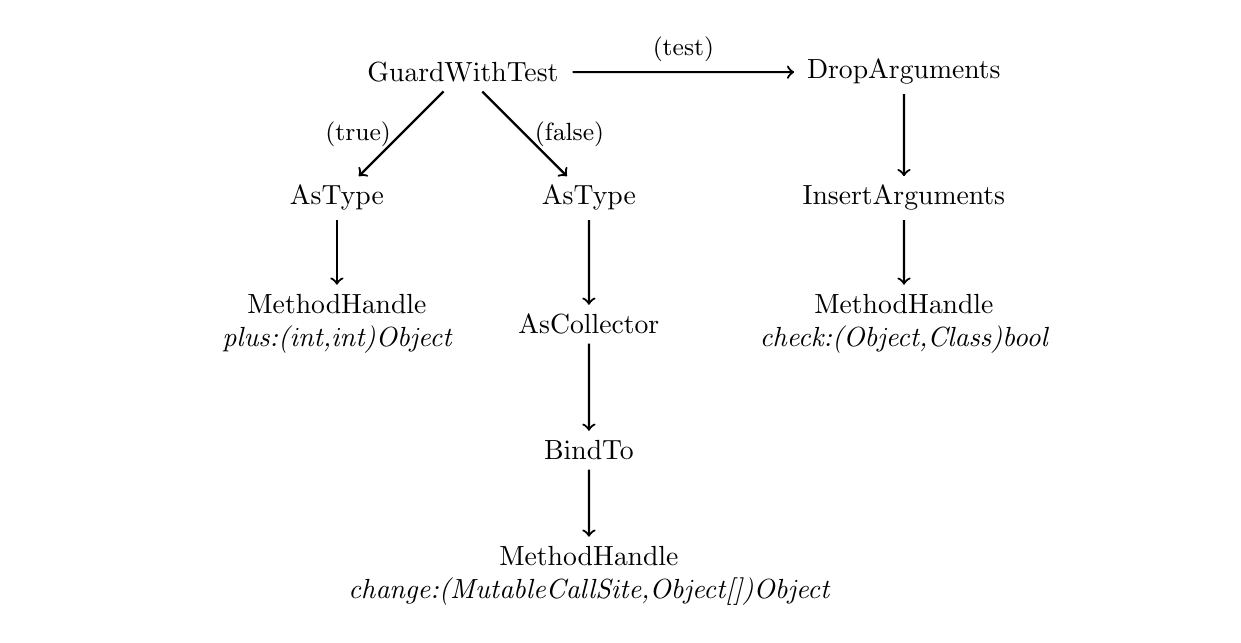
\begin{tikzpicture}[scale=1.6]
  \node[text width=3in,align=center](A1) at (2,-2){AsType};
  \node[text width=3in,align=center](A2) at (2,-3){AsCollector};
  \node[text width=3in,align=center](A3) at (2,-4){BindTo};
  \node[text width=3in,align=center](A4) at (2,-5){MethodHandle\\{\it change:(MutableCallSite,Object[])Object}};

  \node[text width=1in,align=center](G1) at (1,-1){GuardWithTest};

  \node[text width=3in,align=center](B1) at (0,-2){AsType};
  \node[text width=3in,align=center](B2) at (0,-3){MethodHandle\\{\it plus:(int,int)Object}};

  \node[text width=1in,align=center](C1) at (4.5,-1){DropArguments};
  \node[text width=3in,align=center](C2) at (4.5,-2){InsertArguments};
  \node[text width=3in,align=center](C3) at (4.5,-3){MethodHandle\\{\it check:(Object,Class)bool}};

  \draw[thick,->](A1) -- (A2);
  \draw[thick,->](A2) -- (A3);
  \draw[thick,->](A3) -- (A4);
  \draw[thick,->](B1) -- (B2);

  \draw[thick,->](C1) -- (C2);
  \draw[thick,->](C2) -- (C3);
  \draw[thick,->](G1) -- node[right] {\small (false)} (A1);
  \draw[thick,->](G1) -- node[left]  {\small (true)}  (B1);
  \draw[thick,->](G1) -- node[above] {\small (test)}  (C1);
\end{tikzpicture}
}
          \caption{method handles tree: first call (integer)}
          \label{ast2}
        \end{figure}

        If ’a’ is a string, the method ``change'' is called again,
        installing a new method handle tree testing if ’a’ is a string in order to call plus(String,int)Object.
        This adaptation form the method handles tree of the figure \ref{ast3}.

        % graph 3
        \begin{figure*}
          \centering \resizebox{.8\linewidth}{!}{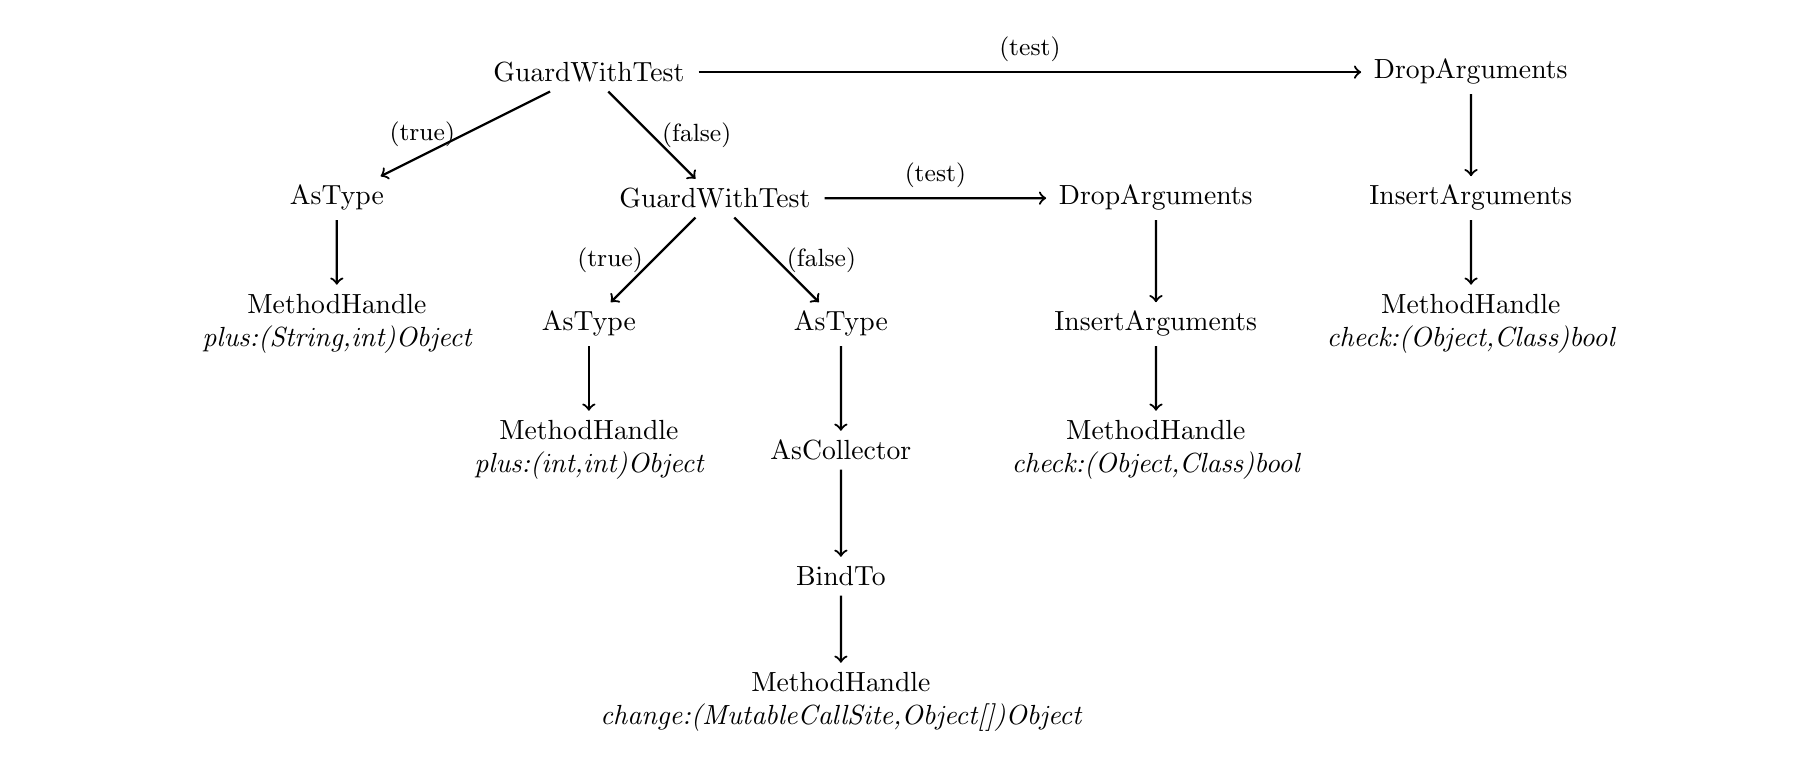
\begin{tikzpicture}[scale=1.6]
    \node[text width=3in,align=center](A1) at (2,-2){AsType};
    \node[text width=3in,align=center](A2) at (2,-3){AsCollector};
    \node[text width=3in,align=center](A3) at (2,-4){BindTo};
    \node[text width=3in,align=center](A4) at (2,-5){MethodHandle\\{\it change:(MutableCallSite,Object[])Object}};

    \node[text width=1in,align=center](G1) at (1,-1){GuardWithTest};

    \node[text width=3in,align=center](B1) at (0,-2){AsType};
    \node[text width=3in,align=center](B2) at (0,-3){MethodHandle\\{\it plus:(int,int)Object}};

    \node[text width=1in,align=center](C1) at (4.5,-1){DropArguments};
    \node[text width=3in,align=center](C2) at (4.5,-2){InsertArguments};
    \node[text width=3in,align=center](C3) at (4.5,-3){MethodHandle\\{\it check:(Object,Class)bool}};

    \node[text width=1in,align=center](G2) at (0, 0){GuardWithTest};

    \node[text width=3in,align=center](D1) at (-2,-1){AsType};
    \node[text width=3in,align=center](D2) at (-2,-2){MethodHandle\\{\it plus:(String,int)Object}};

    \node[text width=1in,align=center](E1) at (7, 0){DropArguments};
    \node[text width=3in,align=center](E2) at (7,-1){InsertArguments};
    \node[text width=3in,align=center](E3) at (7,-2){MethodHandle\\{\it check:(Object,Class)bool}};

    \draw[thick,->](A1) -- (A2);
    \draw[thick,->](A2) -- (A3);
    \draw[thick,->](A3) -- (A4);
    \draw[thick,->](B1) -- (B2);

    \draw[thick,->](C1) -- (C2);
    \draw[thick,->](C2) -- (C3);
    \draw[thick,->](G1) -- node[right] {\small (false)} (A1);
    \draw[thick,->](G1) -- node[left]  {\small (true)}  (B1);
    \draw[thick,->](G1) -- node[above] {\small (test)}  (C1);

    \draw[thick,->](D1) -- (D2);
    \draw[thick,->](E1) -- (E2);
    \draw[thick,->](E2) -- (E3);
    \draw[thick,->](G2) -- node[right] {\small (false)} (G1);
    \draw[thick,->](G2) -- node[left]  {\small (true)}  (D1);
    \draw[thick,->](G2) -- node[above] {\small (test)}  (E1);
\end{tikzpicture}
}
          \caption{method handles tree: second call (string)}
          \label{ast3}
        \end{figure*}


%         \begin{enumerate}
%           \item \textbf{Kinds of MethodHandle}\\
%             The MethodHandle class is composed of different types grouped into 4 kinds,
%             ``constant'', ``bound'', ``invokers'' and ``others''.
%             The three first have many specials paths in the \VM for each instruction.
%             While ``others'' have a unique path.
%           \item \textbf{Contents}\\
%             It contains a type descriptor (methodtype).
%             All instances of MethodHandle are immutable.
%             It have a pair of special invoker methods called invokeExact and invoke.
%             The invokeExact invoker accepts calls which exactly match the method handle's own type.
%         \end{enumerate}

      \subsubsection{CallSite}
        A CallSite is a holder for a variable MethodHandle, which is called its target.
        An invokedynamic instruction linked to a CallSite delegates all calls to the site's current target.
        A CallSite may be associated with several invokedynamic instructions,
        or it may be ``free floating'', associated with none.\\

        It has three immediate, concrete subclasses that may be either instantiated or subclassed.
        \begin{enumerate}
          \item \textbf{ConstantCallSite} : If a mutable target is not required.
          \item \textbf{MutableCallSite}  : If a mutable target is required
          \item \textbf{VolatileCallSite} : If a mutable target is required which has volatile variable semantics.
        \end{enumerate}
        A non-constant call site may be relinked by changing its target.
        The new target must have the same type as the previous target.

      \subsubsection{SwitchPoint}
        The Java bytecode is compiled and optimized on the fly by the JIT compiler.
        However, it may be that the code need to be deoptimize.
        The \JVM contains some ``flags'' which indicate a need to degrade a code.
        So, it can ``drop'' a optimized code to optimize it again.
        it is essential that all threads were aware of changes.
        Using the safe-point (a mechanism of Garbage Collector) is recommended.

        A SwitchPoint is an object allowing this mechanism.
        It indicates that a code must be degraded and synchronizes threads.
        The SavePoint is not necessarily available.
        An alternative is to synchronize all threads with a volatile variable.
        It contains a target method and a fallback method.
%         http://docs.oracle.com/javase/7/docs/api/java/lang/invoke/SwitchPoint.html
        
        
%     \subsubsection{MethodHandle}
%       \label{jsrMH}
%       A method handle is a typed, directly executable reference to
%       an underlying method, constructor, field, or similar low-level operation,
%       with optional transformations of arguments or return values.
% 
% 
%       \begin{enumerate}[A.]
%         \item \textbf{Kinds of MethodHandle}\\
%           The MethodHandle class is composed of different types grouped into 4 kinds,
%           ``constant'', ``bound'', ``invokers'' and ``others''.
%           The three first have many specials paths in the \VM for each instruction.
%           While ``others'' have a unique path.
% 
%           \begin{enumerate}[1.]
%             \item \textbf{Constant}\\
%               The kind ``constant'' contains many instructions:\\
% 
%               \begin{tabular}{c c c}
%                 \begin{minipage}{4cm}
%                   \begin{itemize}
%                     \item invokeVirtual
%                     \item invokeInterface
%                     \item invokeStatic
%                     \item invokeSpecial
%                   \end{itemize}
%                 \end{minipage}
%                 &
%                 \begin{minipage}{4cm}
%                   \begin{itemize}
%                     \item getStatic
%                     \item putStatic
%                     \item getField
%                     \item putField
%                   \end{itemize}
%                 \end{minipage}
%                 &
%                 \begin{minipage}{5cm}
%                   \begin{itemize}
%                     \item invokeDirect (\DALVIK)
%                     \item newInvokeSpecial
%                   \end{itemize}
%                 \end{minipage}
%               \end{tabular}
% 
%             \item \textbf{Bound}\\
%               The kind ``bound'' contains an invoke-virtual \textit{un-virtualized}.
%               It is a MethodHandle constant created with invoke-virtual or invoke-interface
%               and a call to the ``bindTo'' function to bind the receiver.
%               It is equivalent to calling the Dalvik instructions :
%               \textit{invoke-direct} with a constant object on first parameter..
% 
%             \item \textbf{Invoker}
%               \begin{itemize}
%                 \item invoker
%                 \item ExactInvoker
%                 \item VarargCollectorInvoker (?)
%               \end{itemize}
% 
%             \item \textbf{And the others}\\
%               Those are MethodHandle adapters.
%           \end{enumerate}
% 
%         \item \textbf{Contents}\\
%           It contains a type descriptor (methodtype).
%           All instances of MethodHandle are immutable.
%           It have a pair of special invoker methods called invokeExact and invoke.
%           The invokeExact invoker accepts calls which exactly match the method handle's own type.
% 
%           \begin{enumerate}[1.]
%             \item \textbf{invokeExact method}\\
%               The invokeExact method allows to call a method handle with an exact type match.
%               The symbolic type descriptor at the call site of invokeExact
%               must exactly match this method handle's type.
%               No conversions are allowed on arguments or return values.
%               A runtime exception is thrown otherwise.
% 
%             \item \textbf{invoke method}\\
%               The invoke method allows to call a method handle
%               and eventually performing conversions on arguments and return values.
%               It's semantically equivalent to call a method named ``asType'' to convert the type descriptor.
%               This method thrown an ``ClassCastException'' if the conversion is impossible.
%               When the type descriptor and the method handle type descriptor correspond, it calls the invokeExact method.
%           \end{enumerate}
%       \end{enumerate}


    \subsection{Instructions and constants}
      With the \JSR, the \VM have to know new constants and new instructions.
      Two new entries into the constant pool can be done, one for a method type and another for a method handle.

      An only one instruction has been added on top of the \VM, ``invokedynamic''.
      This instruction allows to do a late linker and allows to modify this link at runtime.
      When the \VM reads an ``invokedynamic'' instruction, a bootstrap method, defined in the instruction, is called.
      This method creates a call site for the actual call and the nexts.
      A bootstrap method can take 0 to 251 arguments.

      Two other instructions has been added as native methods, ``invoke'' and ``invokeExact''.
      These instructions handle function pointers (method handle),
      this is why the compiler cannot find the real method to call and cannot find the signature.
      So, the compiler creates the signature corresponding to the actual context
      and assumes that the method (method handle) will be on the stack at runtime.
      This process is called ``method with a polymorphic signature''.

\section{Related Work}

  Currently only the desktop (HotSpot) and the server (J9) version of the JVM have a complete implementation of the JSR 292.
  These implementations use mechanisms that we cannot reuse with Dalvik (code generation, rewriting, \dots)
  because of the power costs and computing restrictions.
  So, Dalvik is seen like a specific virtual machine from language developers.
    
  Our solution is to make an implementation of the JSR 292 for Android.
  But, because Android have many constraints from its environment,
  we have to reinterpret the JSR.
  The API is the same, but not the VM specification.
    
  To do this, we made a new DEX format with new instructions, new constants, \dots
  And we made an specific interpreter, written in Java, which execute method handle trees (combiners).

\section{A new DEX format}

  New instructions and new constants imply a new format of the DEX file.
  We enhance the opcode set, add constant-pools and change the header of classes.
  But we have to maintained the compatibility with the pre-JSR 292 APK files.

  \subsection{opcodes / constants}
    The \JSR needs two new constants (``const-methodtype'' and ``const-methodhandle'') and a new instruction (``invoke-dynamic'').
    Regarding the two methods ``invoke'' and ``invokeExact'', we do the choice to add two new instructions:
    ``invoke-exact'' for the ``invokeExact'' method and ``invoke-generic'' for the ``invoke'' method (that avoids all possible mix-ups with the reflection API).

  \subsection{constant-pools}

    Dalvik have a constant pool for each entry type.
    So we have to add four constant pools (fig. \ref{SNA}), one for each entry we need
    (MethodType, MethodHandle, InvokeDynamic and Bootstrap Arguments).

    \begin{figure}[!h]
      \centering \includegraphics[width=.5\columnwidth]{structure-apk-292.png}
      \caption{structure of new APK files}
      \label{SNA}
    \end{figure}

    The MethodType entry contains an index into the prototype constant pool.
    The MethodHandle entry contains the method handle kind (cf. \ref{MH})
    and an index into the method or the field constant pool, according to the kind.
    The InvokeDynamic entry contains indexes into the string, the prototype,
    the method handle and the bootstrap arguments constant pools.
    And the Bootstrap arguments entry contains its arguments number
    and a data block representing the arguments.
    Each argument is encoded with a tag
    followed by a constant pool index or the primitive value according to the tag.
%    (fig. \ref{DVMstruct}).

%    \begin{figure}[!h]
%      \centering {\scriptsize \begin{verbatim}
  /* Direct-mapped "methodType_id_item". */
  struct DexMethodTypeId {
    u2  protoIdx;     /* index into protoIds */
  };
\end{verbatim} }

%      \centering {\scriptsize \begin{verbatim}
  /*
   * Direct-mapped "methodHandle_id_item".
   */
  struct DexMethodHandleId {
    u4  kind;
    u4  memberIdx;    /* index into methodIds or fieldIds */
  };
\end{verbatim} }

%      \centering {\scriptsize \begin{verbatim}
  /*
   * Direct-mapped "indy_id_item".
   */
  struct DexInvokeDynamicId {
    u4 nameIdx;       /* index into stringIdx */
    u2 typeIdx;       /* index into protoIdx */
    u2 methodHandleIdx;
    u4 bsmargOff;
  };
\end{verbatim} }

%      \centering {\scriptsize \begin{verbatim}
  /* Direct-mapped "bsmArgsList_id_item". */
  struct DexBsmArgsListId {
    u4 size;          /* number of argument couples */
    u1 arguments[1];  /* array of couple {type,[idx|value]} */
  };
\end{verbatim} }

%      \caption{MethodType, MethodHandle, InvokeDynamic and Bootstrap arguments constant pool entries}
%      \label{DVMstruct}
%    \end{figure}

      {\scriptsize \begin{verbatim}
  /* Direct-mapped "methodType_id_item". */
  struct DexMethodTypeId {
    u2  protoIdx;     /* index into protoIds */
  };
\end{verbatim} }

      {\scriptsize \begin{verbatim}
  /*
   * Direct-mapped "methodHandle_id_item".
   */
  struct DexMethodHandleId {
    u4  kind;
    u4  memberIdx;    /* index into methodIds or fieldIds */
  };
\end{verbatim} }

      {\scriptsize \begin{verbatim}
  /*
   * Direct-mapped "indy_id_item".
   */
  struct DexInvokeDynamicId {
    u4 nameIdx;       /* index into stringIdx */
    u2 typeIdx;       /* index into protoIdx */
    u2 methodHandleIdx;
    u4 bsmargOff;
  };
\end{verbatim} }

      {\scriptsize \begin{verbatim}
  /* Direct-mapped "bsmArgsList_id_item". */
  struct DexBsmArgsListId {
    u4 size;          /* number of argument couples */
    u1 arguments[1];  /* array of couple {type,[idx|value]} */
  };
\end{verbatim} }


  \subsection{Class header}

    A call site is bound to an instruction so it's not interresting to store them into a constant-pool.
    So we have to create a table that contains the call sites.
    We have three ways to store the call sites: in the DEX header; in the method which contains the instruction or in the class where the method is.
    As a reminder, a DEX file contains whole the classes from a program, and a class can contains at most 65535 methods (cf. jvms 4.11).
    A method can contains a lot of instructions so the table of call sites can quickly overflow.
    The best solution is to store the call sites in the method, but Dalvik don't have a lazy mecanism to create methods.
    All methods are created when the class was created.
    So we take on the solution where a table is store in the header of each class.

  \subsection{Pre-JSR compatibility}
    Our \ANDROID version understands post-invokedynamic APK.
    We need to modify the APK to add missing constant pools and CallSite tables.
    However an APK is read-only.
    But the installation time does optimizations and has to modify the APK.
    So we take advantage to the installation time to add our work.
    We just simulate an APK without MethodHandle, MethodType, CallSite, \dots
    Only the DEX header and classes header change, we add empty constant pools to the header
    and an empty table to each class representing the CallSite table.
    No offset changes, just the size of header and classes.

\section{New constants}

  We can create constant method handles only with a LDC instruction or in the arguments of a bootstrap method.
  The method handle LDC instruction are rarely used and a bootstrap method is called once.
  So it's not necessary to have a cache for method handles resolved.
  Resolve a method handle consist of find its informations into the constant-pool and create it.
  This creation can only do in Java so an up call is necessary.

  Comparing method types is common on the VM.
  To simplify and optimize these tests, we need to maintain a cache which make sure that two method types with the same signature are identicals.
  A method type can be create in Java or by the VM so the cache run in Java and only Java can create a method type.
  All method types are store in the cache and a test between two method types becomes a simply equality test.
  Resolve a method type consist of find it prototype in the constant-pool and call Java to find it or create it.
  We distinguish two types of method type: some are used by the VM (strong) and mustn't be freed by the GC; the others (weak) can be freed by the GC if necessary.

  \begin{figure}[!h]
    \centering \begin{tabular}{|c|c|c|}
  \hline
  \tinyline{opcode}{format}{description}
  \tinyline
    {3e}{21c}
    {%
      \begin{listminimal}{6cm}
        \item const-methodtype vA, methodtype$@$BBBB
          \item \hspace{.2in}A : destination register or pair (4 bits)
          \item \hspace{.2in}B : methodtype reference index (16 bits)
      \end{listminimal}
    }
  \tinyline
    {3f}{21c}
    {%
      \begin{listminimal}{6cm}
        \item const-methodhandle vA, methodhandle$@$BBBB
          \item \hspace{.2in}A : destination register or pair (4 bits)
          \item \hspace{.2in}B : methodhandle reference index (16 bits)
      \end{listminimal}
    }
\end{tabular}

    \caption{methodtype and methodhandle ldc (load constant)}
    \label{MTMHldc}
  \end{figure}

\section{New invoke instructions}
  All new instructions work with a method handle so we made a method which treats a method handle.
  It invokes the method, get or set a field or call the interpret depending to the kind of the method handle.
  This method is called ``invokeMethodHandle''.
  
  Each instruction have two representation: a ``normal'' form and a ``range'' form.
  The ``normal'' form represents the instruction with at most 5 registers.
  And the ``range'' form can have at most 65535 registers.
  Each register is considered 32 bits wide.

  \subsection{invoke-exact}

    invoke-exact is the instructions with the most simple implementation.
    An invoke-exact contains a index in the constant-pool of method types.
    This method type represents the order and types of the arguments passed to the instruction, the first argument excluded.
    The first argument is the method handle we have to call.
    If the two method types (contained in the instruction and in the method handle) are equals, we call the method handle.
    Else an exception is thrown.

  \subsection{invoke-generic}

    invoke-generic works like an invoke-exact but if the method types differ, we try to adapt arguments.
    Differents treatment can be done:
    if the number of arguments is the same between the two method types, we try to convert arguments;
    else if we have a variadic signature, we collect and convert arguments to match the method type of the method handle.
    else an exception is thrown.
    When the arguments match the method signature, we call the method handle.

    \begin{figure}[!h]
      \centering \begin{tabular}{|c|c|c|}
  \hline
  \tinyline{opcode}{format}{description}
  \tinyline
    {40..41}{35c}
    {
      \begin{listminimal}{6cm}
        \item invoke-\textit{kind} \{vC, vD, vE, vF, vG\}, methodtype$@$BBBB
          \item \hspace{.1in}40 : invoke-exact
          \item \hspace{.1in}41 : invoke-generic
            \item \hspace{.2in}A : argument word count (4 bits)
            \item \hspace{.2in}B : methodtype reference index (16 bits)
            \item \hspace{.2in}C..G : argument registers (4 bits each)
      \end{listminimal}
    }
  \tinyline
    {42..43}{3rc}
    {
      \begin{listminimal}{6cm}
        \item invoke-\textit{kind}/range \{vCCCC .. vNNNN\}, methodtype$@$BBBB
          \item \hspace{.1in}42 : invoke-exact/range
          \item \hspace{.1in}43 : invoke-generic/range
            \item \hspace{.2in}A : argument word count (8 bits)
            \item \hspace{.2in}B : methodtype reference index (16 bits)
            \item \hspace{.2in}C : first argument register (16 bits)
            \item \hspace{.2in}N = A + C - 1
      \end{listminimal}
    }
\end{tabular}

      \caption{invoke-generic/exact instruction}
      \label{INGEins}
    \end{figure}

  \subsection{invoke-dynamic}

    An invoke-dynamic contains a index in the constant-pool of invoke-dynamic and un integer corresponding to the call site number.

    \begin{figure}[!h]
      \centering \begin{tabular}{|c|c|c|}
  \hline
  \tinyline{opcode}{format}{description}
  \tinyline
    {73}{55ci}
    {
      \begin{listminimal}{6cm}
        \item 73 : invoke-dynamic \{vC, vD, vE, vF, vG\},
        \item \hspace{.6in} indy$@$BBBB, \#ZZZZZZZZ
          \item \hspace{.2in}A:C-G : like invoke-exact and invoke-generic
          \item \hspace{.2in}B : invoke-dynamic reference index (16 bits)
          \item \hspace{.2in}Z : callsite\_index (32 bits)
      \end{listminimal}
    }
  \tinyline
    {79}{5rci}
    {
      \begin{listminimal}{6cm}
        \item 79 : invoke-dynamic/range \{vCCCC .. vNNNN\},
        \item \hspace{.6in} indy$@$BBBB, \#ZZZZZZZZ
          \item \hspace{.2in}A:C-N : like invoke-\{exact|generic\}/range
          \item \hspace{.2in}B : invoke-dynamic reference index (16 bits)
          \item \hspace{.2in}Z : callsite\_index (32 bits)
      \end{listminimal}
    }
\end{tabular}

      \caption{invoke-dynamic instruction}
      \label{INDYins}
    \end{figure}

    The call site is found in the current class but if it's the first time we read this instruction, the call site is not created.
    So we need to call the bootstrap method associated to the instruction first.
    So we decode the arguments of the bootstrap method and do an up call to a method called ``callBootstrapMethod'' (fig. \ref{bsm}).
    This method will be detailed after.
    It returns a call site that we store in the class.
    Because this instruction can be read by many threads, we use an atomic ``compare-and-set'' mecanism to store the call site.
    When we have the call site, we get the method handle contains in the call site.
    All method handles are volatiles so we have to get it atomically.
    At the end, we call the method handle.

    \subsection{Implementation details}

      \subsubsection{bootstrap method caller}

        When an ``invoke-dynamic'' is treated, the \JVM call the bootstrap method associated.% (fig. \ref{bsm}).
        A bootstrap method needs at least three arguments:
        a lookup (Lookup), that it's a security token object encapsulating access rigths of class containing the invoke-dynamic opcode;
        an arbitrary name (String) specified as parameter of the invoke-dynamic opcode;
        a method type (MethodType), that it's a reified object of the descriptor specified as parameter of the invoke-dynamic opcode;
        and any constant values specified as bootstrap arguments of the invoke-dynamic opcode.

%      \begin{figure}[!h]
        {\tiny \begin{verbatim}
  private static CallSite callBootstrapMethod(MethodHandle methodHandle, Class<?> lookupClass,
                                          String indyName, MethodType indyType,
                                          Object[] bootstrapArguments) throws Throwable {
    MethodHandles.Lookup lookup = new MethodHandles.Lookup(MethodHandles.Lookup.PRIVATE, lookupClass);
    CallSite callSite;
    try {
      if (bootstrapArguments == null) {  // fast path
        callSite = (CallSite) methodHandle.invokeExact(lookup, indyName, indyType);
      } else {
        Object[] args = new Object[3 + bootstrapArguments.length];
        args[0] = lookup;
        args[1] = indyName;
        args[2] = indyType;
        System.arraycopy(bootstrapArguments, 0, args, 3, bootstrapArguments.length);
        callSite = (CallSite) methodHandle.invokeWithArguments(args);
      }
    } catch (WrongMethodTypeException e) {
      throw new BootstrapMethodError(e);
    }
    if (callSite == null) {
      throw new BootstrapMethodError("callsite is null");
    }
    Object mhOrType = callSite.target;
    if (mhOrType == null) {
      throw new BootstrapMethodError("callsite.target is null");
    }
    if (!(mhOrType instanceof MethodHandle)) {
      throw new BootstrapMethodError("callsite.target is not initialized");
    }
    MethodHandle target = (MethodHandle) mhOrType;
    if (target.type() != indyType) {
      throw new BootstrapMethodError(
          new WrongMethodTypeException("target.type " + target.type() + " type " + indyType));
    }
    return callSite;
  }
\end{verbatim} }
%        \caption{Code of bootstrap method invoker}
%        \label{bsm}
%      \end{figure}

        At first, we have to create the lookup from the declaring class given.
        We treat the bootstrap method differently if arguments are given or not.
        If no arguments are given, we call directly the bootstrap method
        with an ``invokeExact'' and the basic arguments (types are known).

        Else, we add the basic arguments into the other arguments
        and because arguments are seen like an array of Object,
        we have to call the ``invoke'' method.
        The ``invoke'' method needs the true signature when we call it,
        so we have to dispatch arguments to create the real signature.
        To do that, we call the method ``invokeWithArguments''% (fig. \ref{IWA})
        which call the method invoke according to the number of arguments.
        ``invokeWithArguments'' is separated on many functions to allow optimizations by the JIT.

        {\tiny \begin{verbatim}
  public Object invokeWithArguments(Object... arguments) throws Throwable {
    switch (arguments.length) {
      case 0: case 1: case  2: case  3: case  4: case  5: case  6: case  7: case  8:
      case 9: case 10: case 11: case 12: case 13: case 14: case 15: case 16:
        return invokeWithLessThan17Arguments(arguments);
      case 17: case 18: case 19: case 20: case 21: case 22: case 23: case 24:
      case 25: case 26: case 27: case 28: case 29: case 30: case 31: case 32:
        return invokeWithLessThan33Arguments(arguments);
          ...
      default:
        throw new ClassFormatError("Too many arguments (" + arguments.length + ")");
    }
  }

  private Object invokeWithLessThan17Arguments(Object... arguments) throws Throwable {
    switch(arguments.length) {
      case 0:
        return this.invoke();
      case 1:
        return this.invoke(arguments[0]);
      case 2:
        return this.invoke(arguments[0], arguments[1]);
          ...
      default:
        throw new ClassFormatError("Too many arguments (" + arguments.length + ")");
    }
  }
\end{verbatim} }


        When the callsite is returned, we verify the integrity of the callsite.
        We check if it or its target isn't null and if the target's type and the type given are the same.
        Because the target callsite could be uninitialized we have to check if the target contains a method handle or a method type.

%      \begin{figure}[!h]
%        {\tiny \begin{verbatim}
  public Object invokeWithArguments(Object... arguments) throws Throwable {
    switch (arguments.length) {
      case 0: case 1: case  2: case  3: case  4: case  5: case  6: case  7: case  8:
      case 9: case 10: case 11: case 12: case 13: case 14: case 15: case 16:
        return invokeWithLessThan17Arguments(arguments);
      case 17: case 18: case 19: case 20: case 21: case 22: case 23: case 24:
      case 25: case 26: case 27: case 28: case 29: case 30: case 31: case 32:
        return invokeWithLessThan33Arguments(arguments);
          ...
      default:
        throw new ClassFormatError("Too many arguments (" + arguments.length + ")");
    }
  }

  private Object invokeWithLessThan17Arguments(Object... arguments) throws Throwable {
    switch(arguments.length) {
      case 0:
        return this.invoke();
      case 1:
        return this.invoke(arguments[0]);
      case 2:
        return this.invoke(arguments[0], arguments[1]);
          ...
      default:
        throw new ClassFormatError("Too many arguments (" + arguments.length + ")");
    }
  }
\end{verbatim} }

%        \caption{Code of invokeWithArguments}
%        \label{IWA}
%      \end{figure}

      \subsubsection{Method handle (combinor) interpreter}

        The method handle interpreter written in Java% (fig. \ref{intepret})
        is used to interpret method handle trees which start by a combiner.
        It is implemented using a continuation mechanism (context) to treat the return value.
        Each combiner execute its own code and can produce a 'context'.
        For example, AsType converts arguments and produces a context if it has to convert the return value.
        So when the interpreter treats a 'final' method handle,
        which means a method handle produced by a call to 'lookup.findXXX(\dots)' (instance, static, getter, \dots),
        it does an invoke-generic and check if a context exist.
        If there is a context, the interpreter execute the second part of the method handle,
        convert the return value in the case of AsType.
        Afterwards, the interpreter repeats the loop.

        {\tiny \begin{verbatim}
private static Object invokeCombiner(MethodHandle mh, Object[] arguments) throws Throwable {
  ContextInterpret contexts = null;
  main_loop: for (;;) {
    if (mh.getClass() == MethodHandle.class) {
      // method handle produced by a lookup.findXXX()
      Object result = mh.invokeWithArguments(arguments);
      for (;;) {
        if (contexts != null) {
          ContextInterpret context = contexts;
          contexts = contexts.previous;
          switch (context.kind) {
            case AS_TYPE: { ... }
            case GWT: { ... }
            case FOLD_ARGUMENTS: { ... }
            default:
              throw new InternalError("shouldn't happen !");
          }
        }
        return result;
      }
    }
    // combiners
    MHInterpret cmh = (MHInterpret) mh;
    switch (cmh.interpretKind) {
      case BIND_OBJECT: { ... }
      case AS_TYPE: { ... }
      case AS_COLLECTOR: { ... }
      case AS_SPREADER: { ... }
      case GWT: { ... }
      case DROP_ARGUMENTS: { ... }
      case INSERT_ARGUMENTS: { ... }
      case FOLD_ARGUMENTS: { ... }
        ...
      default:
        throw new InternalError("shouldn't happen !");
    }
  }
}
\end{verbatim} }
    
        This implementation avoids to pile up a call in the stack for each method handle.
        We pile up only if we have a 'final' method handle, which is not a subtree.

%    \begin{figure}[!h]
%      {\tiny \begin{verbatim}
private static Object invokeCombiner(MethodHandle mh, Object[] arguments) throws Throwable {
  ContextInterpret contexts = null;
  main_loop: for (;;) {
    if (mh.getClass() == MethodHandle.class) {
      // method handle produced by a lookup.findXXX()
      Object result = mh.invokeWithArguments(arguments);
      for (;;) {
        if (contexts != null) {
          ContextInterpret context = contexts;
          contexts = contexts.previous;
          switch (context.kind) {
            case AS_TYPE: { ... }
            case GWT: { ... }
            case FOLD_ARGUMENTS: { ... }
            default:
              throw new InternalError("shouldn't happen !");
          }
        }
        return result;
      }
    }
    // combiners
    MHInterpret cmh = (MHInterpret) mh;
    switch (cmh.interpretKind) {
      case BIND_OBJECT: { ... }
      case AS_TYPE: { ... }
      case AS_COLLECTOR: { ... }
      case AS_SPREADER: { ... }
      case GWT: { ... }
      case DROP_ARGUMENTS: { ... }
      case INSERT_ARGUMENTS: { ... }
      case FOLD_ARGUMENTS: { ... }
        ...
      default:
        throw new InternalError("shouldn't happen !");
    }
  }
}
\end{verbatim} }
%      \caption{Code of method handles (combiners) interpreter}
%      \label{intepret}
%    \end{figure}

\section{Conclusion}

\appendix
\section{Appendix Title}

This is the text of the appendix, if you need one.

\acks

Acknowledgments, if needed.

% We recommend abbrvnat bibliography style.

\makeatletter
  \def\@seccntformat#1{Appendix~\csname the#1\endcsname:\quad}
\makeatother

\bibliographystyle{abbrvnat}

% The bibliography should be embedded for final submission.

\begin{thebibliography}{}
  \softraggedright

  \bibitem{idc-website}
  IDC website (2013) - \\ \url{www.idc.com/getdoc.jsp?containerId=prUS24257413}

  \bibitem{lang-groovy}
  Groovy website - \\ \url{http://groovy.codehaus.org/}
  
  \bibitem{wiki-android}
  \ANDROID (Wikipedia) - \\ \url{en.wikipedia.org/wiki/Android\_(operating\_system)#Linux}

  \bibitem{wiki-jvm-lang}
  \JVM languages (Wikipedia) - \\ \url{https://en.wikipedia.org/wiki/List\_of\_JVM\_languages}
%   @ARTICLE{5676144, 
%   author={Butler, M.}, 
%   journal={Pervasive Computing, IEEE}, 
%   title={Android: Changing the Mobile Landscape}, 
%   year={2011}, 
%   volume={10}, 
%   number={1}, 
%   pages={4-7}, 
%   keywords={mobile computing;mobile radio;operating systems (computers);Android phones;Google;iPhone market;mobile landscape;smart phones;Androids;Driver circuits;Marketing and sales;Mobile communication;Smart phones;Android;App Inventor for Android;Apple App Store;BlackBerry;Technovation;iPhone}, 
%   doi={10.1109/MPRV.2011.1}, 
%   ISSN={1536-1268},}
  \bibitem{ieee-butler-android-landscape}
   Butler, M., ``Android: Changing the Mobile Landscape,'' Pervasive Computing, IEEE , vol.10, no.1, pp.4,7, Jan.-March 2011

%   @INPROCEEDINGS{5578292, 
%   author={Paul, K. and Kundu, T.K.}, 
%   booktitle={Computer and Information Technology (CIT), 2010 IEEE 10th International Conference on}, 
%   title={Android on Mobile Devices: An Energy Perspective}, 
%   year={2010}, 
%   pages={2421-2426}, 
%   keywords={Java;Linux;energy consumption;mobile handsets;operating system kernels;program compilers;public domain software;Android;Angstrom linux;Dalvik JVM;Google;HTC;JAVA applications;Motorola;OHA;Sun;dynamic compiler;embedded devices;energy consumption;energy perspective;linux kernel;mobile devices;open handset alliance;open source platform;power management framework;Computers;Conferences;Information technology;Android Energy;Dalvik JVM}, 
%   doi={10.1109/CIT.2010.416},}
  \bibitem{ieee-paul-kundu-energy-perspective}
  Paul, K.; Kundu, T.K., ``Android on Mobile Devices: An Energy Perspective,'' Computer and Information Technology (CIT), 2010 IEEE 10th International Conference on , vol., no., pp.2421,2426, June 29 2010-July 1 2010

  \bibitem{ieee-paulson-shift-dynamic-languages}
  Paulson, L.D., ``Developers shift to dynamic programming languages,'' Computer , vol.40, no.2, pp.12,15, Feb. 2007

%   \bibitem[Smith et~al.(2009)Smith, Jones]{smith02}
%   P. Q. Smith, and X. Y. Jones. ...reference text...

\end{thebibliography}


\end{document}

%                       Revision History
%                       -------- -------
%  Date         Person  Ver.    Change
%  ----         ------  ----    ------

%  2013.06.29   TU      0.1--4  comments on permission/copyright notices

